% This file was created with tikzplotlib v0.10.1.
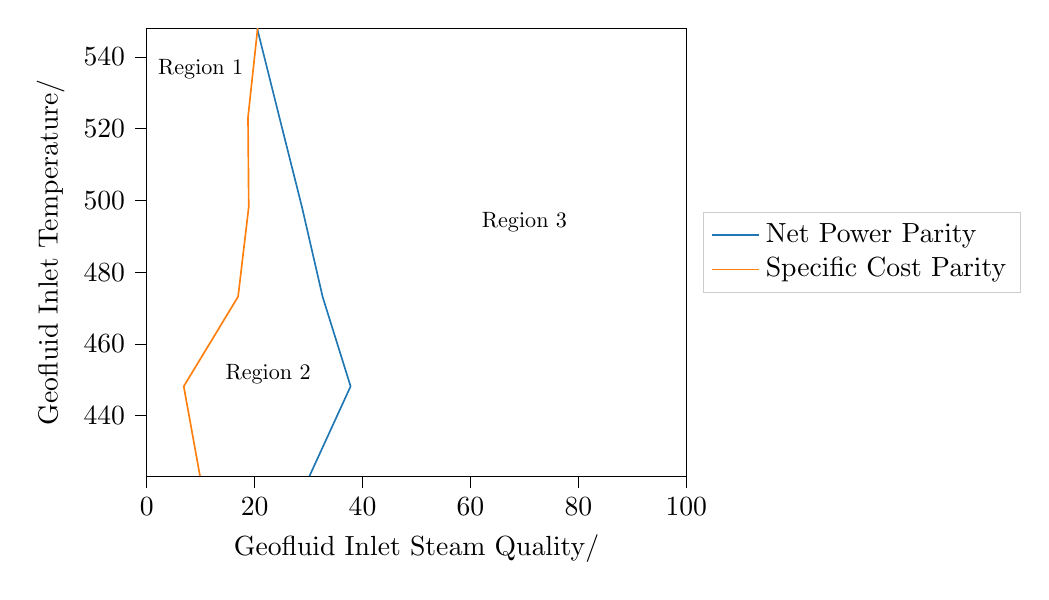
\begin{tikzpicture}

\definecolor{darkgray176}{RGB}{176,176,176}
\definecolor{darkorange25512714}{RGB}{255,127,14}
\definecolor{lightgray204}{RGB}{204,204,204}
\definecolor{steelblue31119180}{RGB}{31,119,180}

\begin{axis}[
legend cell align={left},
legend style={fill opacity=0.8, draw opacity=1, text opacity=1, draw=lightgray204, at={(1.03, 0.5)}, anchor=west},
tick align=outside,
tick pos=left,
x grid style={darkgray176},
xlabel={Geofluid Inlet Steam Quality/\unit{\percent}},
xmin=0, xmax=100,
xtick style={color=black},
y grid style={darkgray176},
ylabel={Geofluid Inlet Temperature/\unit{\K}},
ymin=423, ymax=548,
ytick style={color=black}
]
\addplot [semithick, steelblue31119180]
table {%
30.1732199888322 423.15
37.7893009240293 448.15
32.5990272774492 473.15
28.7760448540457 498.15
24.595078256838 523.15
20.4394782095746 548.15
};
\addlegendentry{Net Power Parity}
\addplot [semithick, darkorange25512714]
table {%
9.88043234136831 423.15
6.87102869593706 448.15
16.9397882658249 473.15
18.9121530717588 498.15
18.7789988175102 523.15
20.5758201963607 548.15
};
\addlegendentry{Specific Cost Parity}
\draw (axis cs:70,492.5) node[
  scale=0.8,
  anchor=base,
  text=black,
  rotate=0.0
]{Region 3};
\draw (axis cs:22.5,450) node[
  scale=0.8,
  anchor=base,
  text=black,
  rotate=0.0
]{Region 2};
\draw (axis cs:10,535) node[
  scale=0.8,
  anchor=base,
  text=black,
  rotate=0.0
]{Region 1};
\end{axis}

\end{tikzpicture}
